\documentclass[12pt, aspectratio=169]{beamer}

\input{../header}
\usepackage{booktabs}

\title{Basics of Hypothesis Testing}
\author{Md. Aminul Islam Shazid}
\date{}


\begin{document}
    {
		\setbeamertemplate{footline}{}
		\addtocounter{framenumber}{-2}

		\begin{frame}
			\titlepage
		\end{frame}

		\begin{frame}{Outline}
            \vfill
			\tableofcontents[subsectionstyle=hide]
            \vfill
		\end{frame}
	}

    \section{Introduction}


    \begin{frame}{Test of Hypothesis - Overview}
        \begin{itemize}
            \item A statistical hypothesis is a claim about a population parameter
            \item We test this claim using sample data
            \item The goal is to make a decision under uncertainty
            \item Decisions are made using probability and sampling distributions
        \end{itemize}
    \end{frame}


    \begin{frame}{Statistical Hypotheses}
        \begin{itemize}
            \item \textbf{Null hypothesis ($H_0$):} baseline assumption
            \item \textbf{Alternative hypothesis ($H_A$):} competing claim
            \item They are mutually exclusive and exhaustive
            \item Example:
            \[
            H_0: \mu = 100 \quad \text{vs} \quad H_A: \mu \neq 100
            \]
            \item Based on the available data, we either reject the null hypothesis in favor of the alternative or ``fail to reject the null hypothesis"
            \item Therefore, we do not ``accept'' the null hypothesis
        \end{itemize}
    \end{frame}


    \begin{frame}{Types of Alternative Hypotheses}
        \begin{itemize}
            \item Two-tailed:
            \[
            H_A: \mu \neq \mu_0
            \]
            \item Left-tailed:
            \[
            H_A: \mu < \mu_0
            \]
            \item Right-tailed:
            \[
            H_A: \mu > \mu_0
            \]
        \end{itemize}
    \end{frame}


    \section{Testing Procedure}

    \begin{frame}{Test Statistic}
        \begin{itemize}
            \item The test statistic is function of sample data used to test $H_0$
            \item Example (Z-test):
            \[
            Z = \frac{\bar{X} - \mu_0}{\sigma/\sqrt{n}}
            \]
            \item Decision is based on the sampling distribution under $H_0$
        \end{itemize}
    \end{frame}


    \begin{frame}{Sampling Distributions of Test Statistics}
        \begin{itemize}
            \item Different test statistics follow different kinds of sampling distributions
            \item Hypothesis testing relies on those sampling distributions
            \item Assuming that $H_0$ is true, the test statistic follows a known sampling distribution
            \item Example: \(Z = \frac{\bar{X} - \mu_0}{\sigma/\sqrt{n}} \sim N(0,1)\)
            \item This allows us to quantify ``how far'' \(\bar{X}\) is from \(\mu_0\), in other words, ``how unusual" our sample is if the null hypothesis is to be true
            \item If the test statistic indicates that the data in the sample is too unusual for the null hypothesis to be true, then the null hypothesis is rejected
        \end{itemize}
    \end{frame}


    \begin{frame}{How a Test is Performed}
        \begin{itemize}
            \item Suppose we have a hypothesis \(\mu_x = \mu_0\) regarding a random variable \(X\)
            \item We collect the data and compute the sample mean \(\bar{x}\)
            \item We either ``reject" or ``fail to reject'' the \(H_0\) based on how ``far'' \(\bar{x}\) is from \(\mu_0\)
            \item In order to be able to quantify the distance between \(\bar{x}\) and \(\mu_0\) in a statistically meaningful way, we have to ``convert'' the sample mean to a test statistic
            \item Then based on the value of the test statistic and the sampling distribution of the test statistic, a decision regarding the null hypothesis is made
        \end{itemize}
    \end{frame}


    \begin{frame}{Type I Error}
        \begin{itemize}
            \item Rejecting $H_0$ when it is true
            \item Probability of type I error (also known as \emph{level of significance}):
            \[
            \alpha = P(\text{Reject } H_0 \mid H_0 \text{ true})
            \]
            \item Also called false positive
        \end{itemize}
    \end{frame}


    \begin{frame}{Type II Error}
        \begin{itemize}
            \item Failing to reject $H_0$ when it is false
            \item Probability of type II error:
            \[
            \beta = P(\text{Fail to reject } H_0 \mid H_0 \text{ false})
            \]
            \item Also called false negative
        \end{itemize}
    \end{frame}


    \begin{frame}{Errors Summary Table}
        \begin{center}
            \begin{tabular}{c|cc}
                \hline
                & $H_0$ True & $H_0$ False \\
                \hline
                Reject $H_0$ & Type I & Correct \\
                Fail to reject $H_0$ & Correct & Type II \\
                \hline
            \end{tabular}
        \end{center}
    \end{frame}


    \begin{frame}{Level of Significance}
        \begin{itemize}
            \item $\alpha = P(\text{Type I error}) = P(\text{Reject } H_0 \mid H_0 \text{ true})$
            \item Common choices: $0.10,\ 0.05,\ 0.01$
            \item It is essentially our ``tolerance'' for type I error
            \item Smaller choice of $\alpha$ means stricter evidence required
            % \item Confidence level:
            % \[
            % 1 - \alpha
            % \]
        \end{itemize}
    \end{frame}


    \begin{frame}{Rejection Region and Critical Value}
        \begin{itemize}
            \item Define a region in the distribution of the test statistic where $H_0$ is rejected
            \item Based on level of significance $\alpha$
            \item If the value of the test statistic falls inside the rejection region, the \(H_0\) is rejected
            \item If it does not fall in the rejection, we fail to reject the \(H_0\)
            % \item For two-tailed test:
            % \[
            % P(\text{Reject } H_0 \mid H_0 \text{ true}) = \alpha
            % \]
        \end{itemize}
    \end{frame}


    \begin{frame}{General Testing Procedure}
        \begin{itemize}
            \item State $H_0$ and $H_A$
            \item Choose $\alpha$
            \item Select test statistic
            \item Determine the rejection region
            \item Compute the value of the test statistic
            \item Make decision: if the test statistic falls in the rejection region then \(H_0\) is rejected
        \end{itemize}
    \end{frame}


    \section{Visualizing the Test}


    \begin{frame}{Sampling Distribution under the Null Hypothesis}
        \begin{columns}
            \begin{column}{0.5\textwidth}
                Suppose the plot shows the sampling distribution of some test statistic \(Z\).

                \vspace{0.5em}

                Different test statistics have different sampling distribution.

                \vspace{0.5em}

                After obtaining the distribution of the test statistic, a region is determined where the calculated value of the test statistic is unlikely to appear.
            \end{column}
            \begin{column}{0.5\textwidth}
                \begin{center}
                    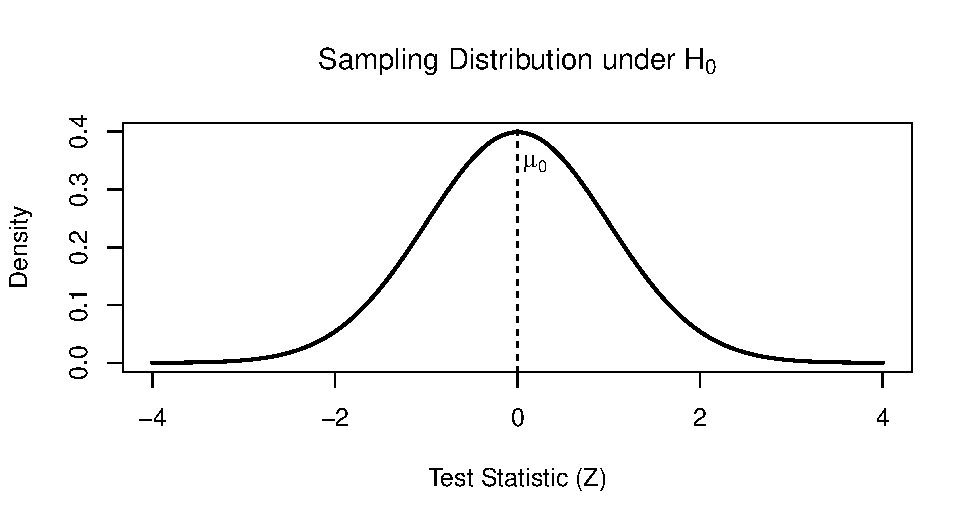
\includegraphics[width=\textwidth]{plots/sampling-dist-under-null.pdf}
                \end{center}
            \end{column}
        \end{columns}
    \end{frame}


    \begin{frame}{Unlikely Region of the Test Statistic under the Null Hypothesis}
        \begin{columns}
            \begin{column}{0.5\textwidth}
                The highlighted region in the plot shows a region of in sampling distribution of the test statistic in which the calculated value of the test staistic is unlikely to fall.

                \vspace{0.5em}

                The question remains as to how to determine this region.

                \vspace{0.5em}

                This region is determined using the level of significance.
            \end{column}
            \begin{column}{0.5\textwidth}
                \begin{center}
                    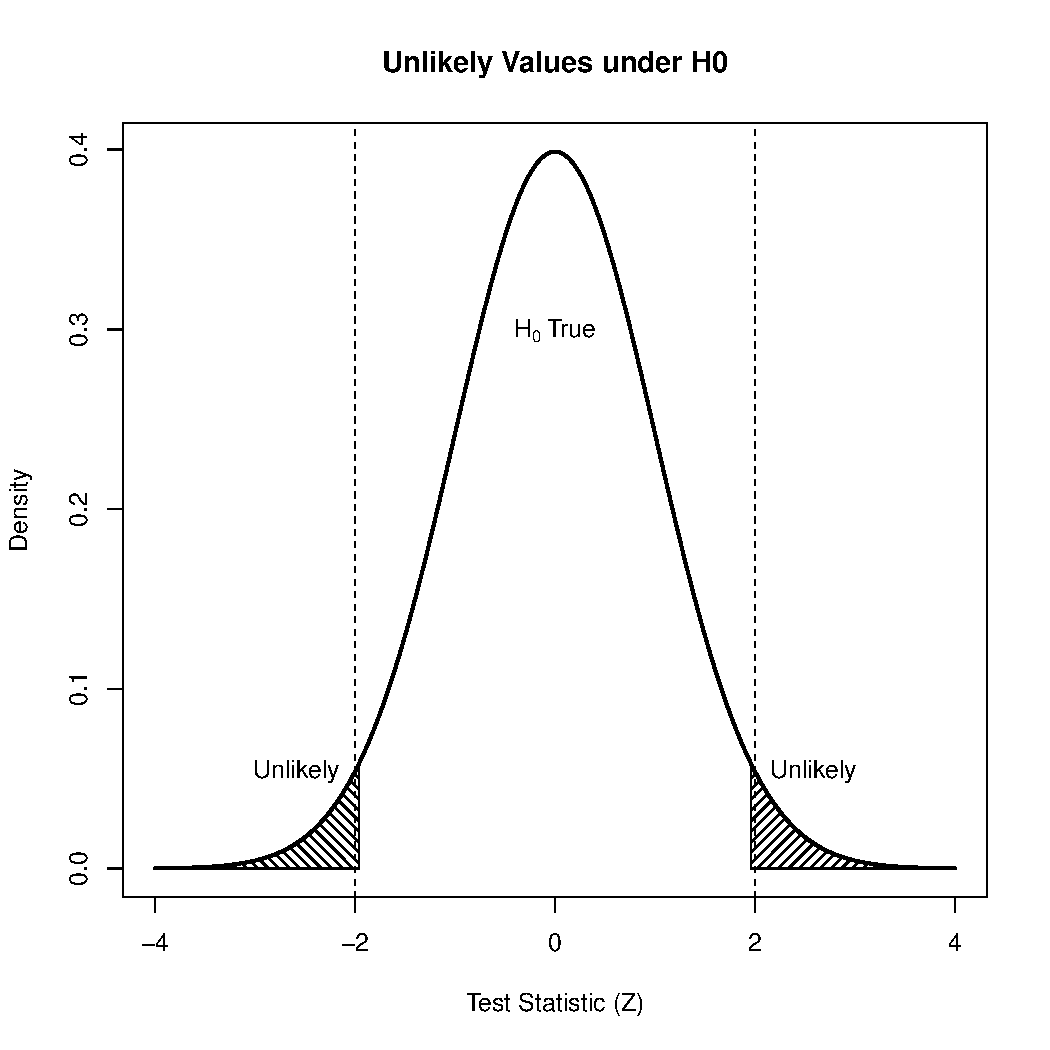
\includegraphics[width=\textwidth]{plots/unlikely-region-under-null.pdf}
                \end{center}
            \end{column}
        \end{columns}
    \end{frame}


    \begin{frame}{Rejection Region in Two-tailed Tests}
        \begin{columns}
            \begin{column}{0.5\textwidth}
                Suppose a value of the ``level of significance, \(\alpha\)" is chosen.

                \vspace{0.5em}

                Then the rejection region is chosen such that the area in the rejection region equals to \(\alpha\).

                \vspace{0.5em}

                Since this is a two-tailed test, the rejection region is on both sides of the distribution and each region has area equal to \(\alpha/2\).

                \vspace{0.5em}

                If the calculated value of the test statistic falls in this region, then the null hypothesis rejected.
            \end{column}
            \begin{column}{0.5\textwidth}
                \begin{center}
                    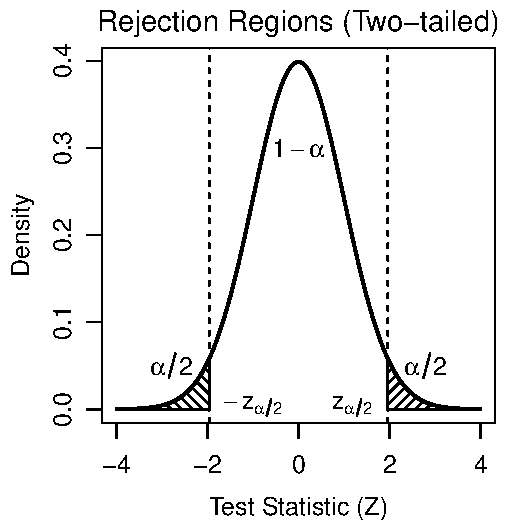
\includegraphics[width=\textwidth]{plots/two-tail-rejection-region.pdf}
                \end{center}
            \end{column}
        \end{columns}
    \end{frame}


    \begin{frame}{Rejection Region in One-tailed Tests}
        \begin{columns}
            \begin{column}{0.5\textwidth}
                \begin{center}
                    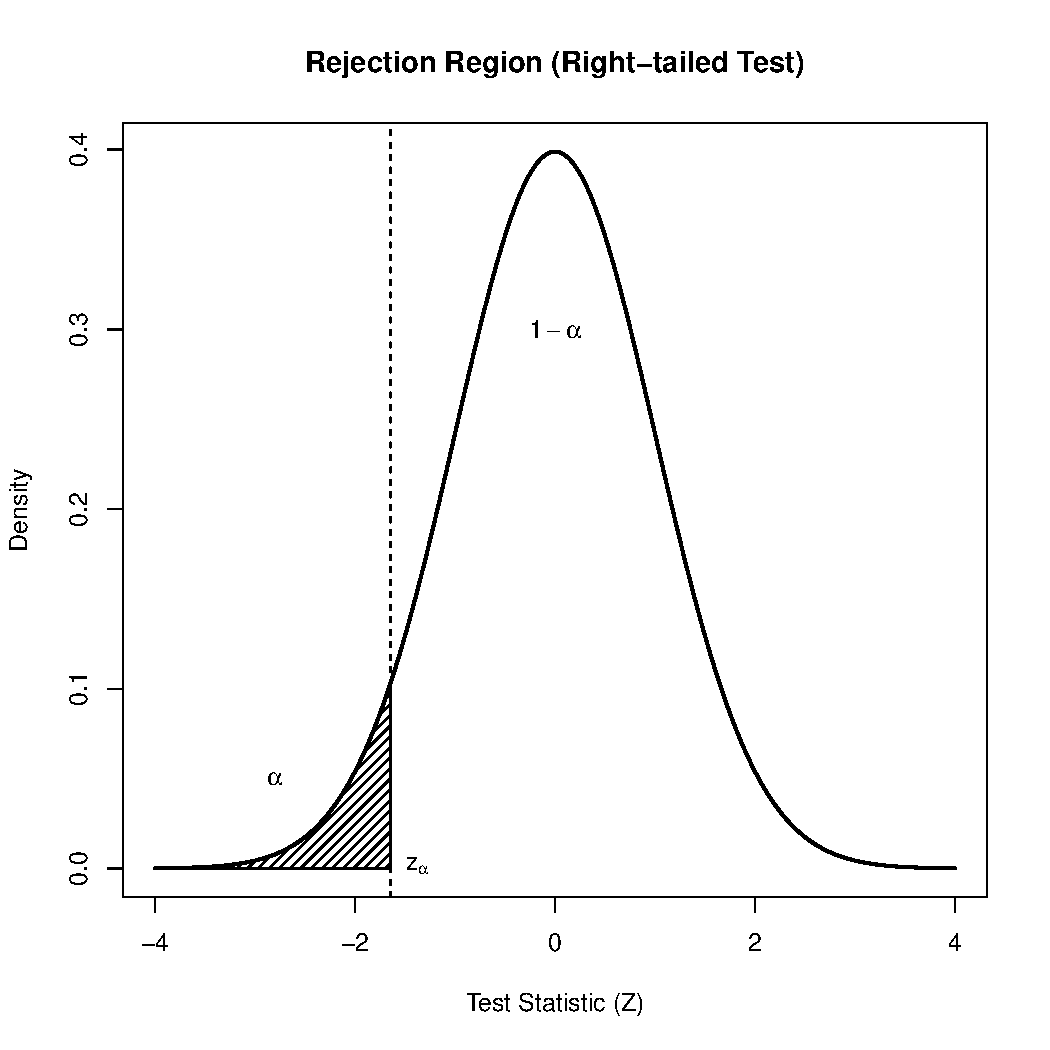
\includegraphics[width=\textwidth]{plots/left-tailed-rejection-region.pdf}
                \end{center}
            \end{column}
            \begin{column}{0.5\textwidth}
                \begin{center}
                    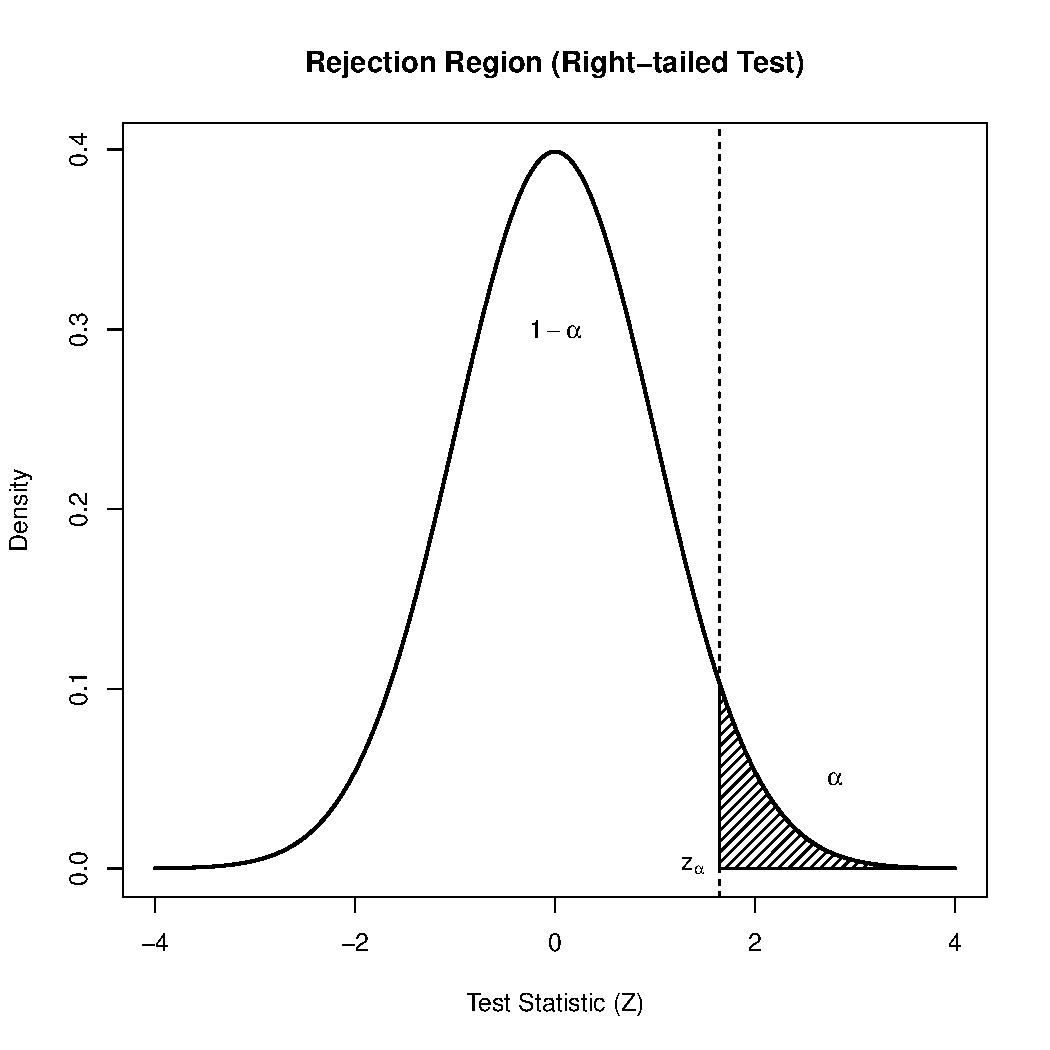
\includegraphics[width=\textwidth]{plots/right-tailed-rejection-region.pdf}
                \end{center}
            \end{column}
        \end{columns}
    \end{frame}


    \begin{frame}{Decision Based on Calculated Value of the Test Statistic}
        \begin{columns}
            \begin{column}{0.5\textwidth}
                \begin{center}
                    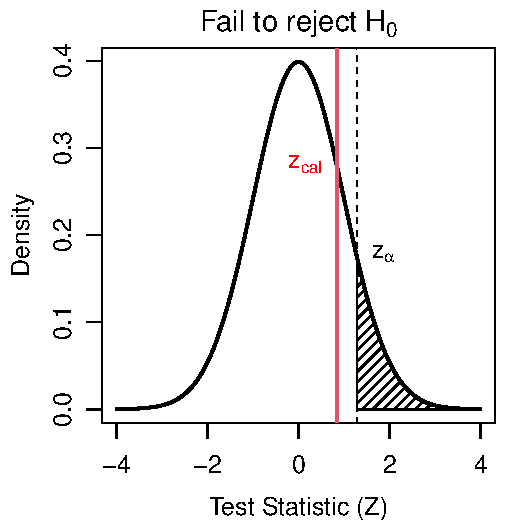
\includegraphics[width=\textwidth]{plots/observed-fail-to-reject.pdf}
                \end{center}
            \end{column}
            \begin{column}{0.5\textwidth}
                \begin{center}
                    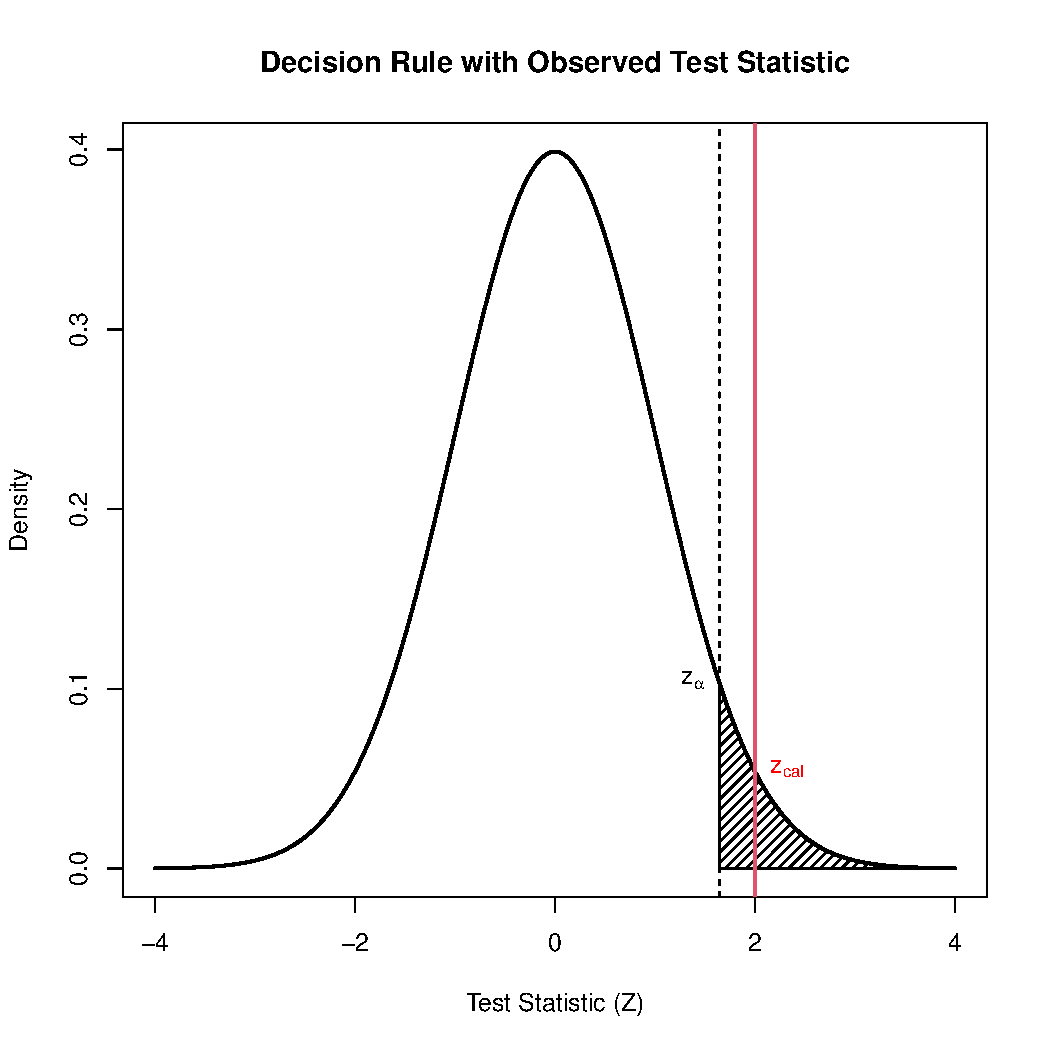
\includegraphics[width=\textwidth]{plots/observed-reject.pdf}
                \end{center}
            \end{column}
        \end{columns}
    \end{frame}


    \section{Power}


    \begin{frame}{Power of a Test}
        \begin{itemize}
            \item \textbf{Power} is the probability of correctly rejecting $H_0$
                when it is actually false
            \[
                \text{Power} = 1 - \beta = P(\text{Reject } H_0 \mid H_0 \text{ false})
            \]
            \item A test with low power may fail to reject a false \(H_0\) which is a \emph{false negative} error
            \item Power depends on:
            \begin{itemize}
                \item \textbf{Sample size} $n$: larger $n$ $\Rightarrow$ higher power
                \item \textbf{Effect size} $|\mu - \mu_0|$: larger effect $\Rightarrow$ easier to detect
                \item \textbf{Variability} $\sigma$: smaller $\sigma$ $\Rightarrow$ higher power
                \item \textbf{Significance level} $\alpha$: larger $\alpha$ $\Rightarrow$ higher power (but at the cost of higher Type I error probability)
            \end{itemize}
            \item Conventionally, power $\geqslant 0.80$ is considered adequate
        \end{itemize}
    \end{frame}


    \begin{frame}{Power: The Two Overlapping Distributions}
        \begin{columns}
            \begin{column}{0.5\textwidth}
                \begin{itemize}
                    \item Under $H_0$: test statistic is centered at $\mu_0$
                    \item Under $H_A$: test statistic is centered at some true $\mu_A \neq \mu_0$
                    \item The \textbf{rejection region} is fixed by $\alpha$ using the $H_0$ distribution
                    \item \textbf{Power} is the area of the $H_A$ distribution
                        that falls \emph{inside} the rejection region
                    \item \textbf{$\beta$} is the area of the $H_A$ distribution
                        that falls \emph{outside} the rejection region
                \end{itemize}
            \end{column}
            \begin{column}{0.5\textwidth}
                \begin{center}
                    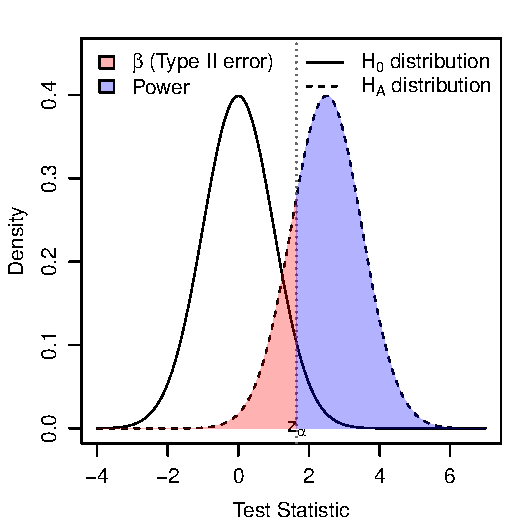
\includegraphics[width=\textwidth]{plots/power-two-distributions.pdf}
                \end{center}
            \end{column}
        \end{columns}
    \end{frame}


    \begin{frame}{Power: The $\alpha$--$\beta$ Trade-off}
        \begin{itemize}
            \item For a fixed sample size, reducing $\alpha$ (stricter test)
                \textbf{moves the rejection region further into the tail}
            \item This means less of the $H_A$ distribution falls in the rejection region
                $\Rightarrow$ power \textbf{decreases} and $\beta$ \textbf{increases}
            \item There is an unavoidable trade-off:
            \begin{center}
                \begin{tabular}{ccc}
                    \toprule
                    $\alpha$ & Type I Error & Power ($1-\beta$) \\
                    \midrule
                    Smaller & Lower  & Lower \\
                    Larger  & Higher & Higher \\
                    \bottomrule
                \end{tabular}
            \end{center}
            \item The only way to reduce \emph{both} errors simultaneously is to
                \textbf{increase the sample size}
            \item In practice, $\alpha$ is fixed first (usually $0.05$),
                then $n$ is chosen to achieve the desired power
        \end{itemize}
    \end{frame}


    \begin{frame}{Test Outcomes and Their Probabilities}
        \begin{center}
            \begin{tabular}{c|cc}
                \hline
                & $H_0$ True & $H_0$ False \\
                \hline
                Reject $H_0$ & Type I ($\alpha$) & Correct ($1-\beta$) \\
                Fail to reject $H_0$ & Correct ($1-\alpha$) & Type II ($\beta$) \\
                \hline
            \end{tabular}
        \end{center}

        \begin{itemize}
            \item \(\alpha = \) level of significance
            \item \(a - \beta = \) power of a test
        \end{itemize}
    \end{frame}


    \section{Example}


    \begin{frame}{Example}
        \begin{itemize}
            \item Claim: teens sleep more than 10 hours
            \item Sample mean: $\bar{x} = 11.5$
            \item $\sigma = 5$, $n = 20$
            \item Hypotheses:
            \[
            H_0: \mu = 10 \quad H_A: \mu > 10
            \]
        \end{itemize}
    \end{frame}


    \begin{frame}{Example Test Statistic}
        \begin{itemize}
            \item Test statistic:
            \[
            Z = \frac{11.5 - 10}{5/\sqrt{20}} = 1.34
            \]
        \end{itemize}
    \end{frame}


    \begin{frame}{Example Decision}
        \begin{itemize}
            \item At $\alpha = 0.05$, the critical value from the sampling distribution of the test statistic, \(z_{0.05}\) is equal to \(1.64\)
            \begin{itemize}
                \item Since $1.34 < 1.64$, we fail to reject $H_0$
            \end{itemize}
            \item At $\alpha = 0.10$, the critical value from the sampling distribution of the test statistic, \(z_{0.10}\) is equal to \(1.28\)
            \begin{itemize}
                \item Since $1.34 > 1.28$, we reject $H_0$
            \end{itemize}
        \end{itemize}
    \end{frame}


    \section{P-value and Confidence Intervals}


    \begin{frame}{P-value}
        \begin{itemize}
            \item The \textbf{p-value} is the probability of observing a test statistic
                as extreme as, or more extreme than, the one calculated from the sample ---
                \emph{assuming $H_0$ is true}
            \item It is \textbf{not} the probability that $H_0$ is true
            \item It quantifies how ``surprising'' or ``unusual'' the data if $H_0$ is to be true
            \item Formally, for a right-tailed test:
            \[
                p = P(Z \geqslant Z_{\text{cal}} \mid H_0 \text{ true})
            \]
            \item Decision rule:
            \begin{itemize}
                \item $p \leqslant \alpha$: reject $H_0$
                \item $p > \alpha$: fail to reject $H_0$
            \end{itemize}
        \end{itemize}
    \end{frame}


    \begin{frame}{P-value Interpretation}
        \begin{itemize}
            \item A \textbf{small} p-value means the observed data would be very
                unlikely if $H_0$ were true, which is evidence against $H_0$
            \item A \textbf{large} p-value means the data are consistent with $H_0$, but this does \emph{not} prove $H_0$ is true. Therefore, we do not ``accept'' the \(H_0\), rather we ``fail to reject it''
            \item Common thresholds (informal):
            \begin{itemize}
                \item $p < 0.10$: some evidence against $H_0$
                \item $p < 0.05$: strong evidence against $H_0$
                \item $p < 0.01$: very strong evidence against $H_0$
            \end{itemize}
            \item \textbf{Common misconceptions:}
            \begin{itemize}
                \item p-value is \emph{not} the probability the result occurred by chance
                \item p-value is \emph{not} a measure of effect size or practical significance
                \item A non-significant p-value does not ``accept'' $H_0$
            \end{itemize}
        \end{itemize}
    \end{frame}


    \begin{frame}{P-value: Tails and Computation}
        \begin{itemize}
            \item The tail(s) used depend on the alternative hypothesis $H_A$:
            \begin{itemize}
                \item Right-tailed ($H_A: \mu > \mu_0$):
                \quad $p = P(Z \geqslant Z_{\text{cal}})$
                \item Left-tailed ($H_A: \mu < \mu_0$):
                \quad $p = P(Z \leqslant Z_{\text{cal}})$
                \item Two-tailed ($H_A: \mu \neq \mu_0$):
                \quad $p = 2\,P(Z \geqslant |Z_{\text{cal}}|)$
            \end{itemize}
            \item \textbf{Example} (from earlier): $Z_{\text{cal}} = 1.34$,\;
                right-tailed test
            \[
                p = P(Z \geqslant 1.34) \approx 0.090
            \]
            \item Since $p = 0.090 > 0.05 = \alpha$, we fail to reject $H_0$ at \(5\%\) of significance
            \item Since $p = 0.090 < 0.10 = \alpha$, we reject $H_0$ at \(10\%\) level of significance
        \end{itemize}
    \end{frame}


    \begin{frame}{Confidence Interval: Construction and Meaning}
        \begin{itemize}
            \item A $100(1-\alpha)\%$ CI is an interval constructed from sample data
                such that, in repeated sampling, it contains the true parameter
                $100(1-\alpha)\%$ of the time
            \item \textbf{Correct interpretation:} if we drew many samples and built a CI
                from each, $(1-\alpha)$ of those intervals would contain $\mu$
            \item \textbf{Incorrect interpretation:} ``there is a $(1-\alpha)$ probability
                that $\mu$ lies in \emph{this} interval'' ---
                $\mu$ is fixed; probability here is a property of the \emph{procedure}
            \item Width of CI:
            \[
                \text{Width} = 2\,z_{\alpha/2}\,\frac{\sigma}{\sqrt{n}}
            \]
            \item Wider CI: less precision; Narrower CI: more precision
            \item Trade-off: higher confidence level $(1-\alpha)\uparrow$
                $\Rightarrow$ wider interval
        \end{itemize}
    \end{frame}


    \begin{frame}{Connection with Confidence Intervals}
        \begin{itemize}
            \item A $100(1-\alpha)\%$ confidence interval for $\mu$ is:
            \[
                \bar{x} \pm z_{\alpha/2}\,\frac{\sigma}{\sqrt{n}}
            \]
            \item A CI gives a \textbf{range of plausible values} for $\mu$,
                whereas a hypothesis test gives a binary decision
            \item The duality: for a two-tailed test at level $\alpha$,
            \[
                \text{Reject } H_0: \mu = \mu_0
                \iff
                \mu_0 \notin \left(\bar{x} - z_{\alpha/2}\tfrac{\sigma}{\sqrt{n}},\;
                                    \bar{x} + z_{\alpha/2}\tfrac{\sigma}{\sqrt{n}}\right)
            \]
            \item \textbf{Advantage of CI over hypothesis test:}
                a CI also communicates the magnitude and precision of the estimate,
                not just whether to reject $H_0$
            \item Narrower CI $\Rightarrow$ more precise estimate
                (achieved by larger $n$ or smaller $\sigma$)
        \end{itemize}
    \end{frame}


    % \begin{frame}{Key Takeaways}
    %     \begin{itemize}
    %         \item Hypothesis testing is decision-making under uncertainty
    %         \item $\alpha$ controls Type I error
    %         \item $\beta$ and power describe sensitivity (probability of detecting a false null hypothesis)
    %         \item P-value provides flexible decision rule
    %         \item Sampling distributions are the foundation
    %     \end{itemize}
    % \end{frame}

    \section*{Thank you.}

\end{document}